\documentclass{article}
\title{Notes for: Learning to Communicate with Deep Multi-Agent Reinforcement Learning}
\author{Michael N.\thanks{paper: https://arxiv.org/abs/1605.06676}}
\date{\today}
\usepackage{graphicx}
\usepackage{dsfont}
\usepackage{amsmath}

\begin{document}
    \maketitle
    \section{High Level and Motivation}

    \subsection{Motivation}

    \paragraph{Switch Riddle}
    

    \emph{
        \begin{enumerate}
            \item After months of evading the police, you have finally been caught and sent to prison.
            \item You are put into a cell, unable to communicate with any of your partners in crime.
            \item Each day the warden selects a prisoner at random and brings them to the interrogation room
            \item The interrogation room contains only a light bulb and a toggle switch
            \item The prisoner can observe the current state of the light bulb and can toggle the light bulb ON/OFF
            \item The prisoner may also announce if they believe all the prisoners have visited the interrogation room
            \item If the prisoner's announcement is true, then all prisoners are set free, but if the announcement is incorrect, all the prisoners are executed.
            \item[When they arrive:] The warden leaves and the prisoners huddle together to discuss their fate. Can they agree on a protocol that will guarantee their freedom?
        \end{enumerate}}

        \paragraph{} Can we enable agents to form communication protocols using deep reinforcement learning?

    \subsection{Problem definition}

    \paragraph{Explicitly} 
    How can we apply an end-to-end deep RL approach to learning:
    fully cooperative, partially observable, sequential multi-agent decision making environments.
    \paragraph{Definitions}
    \begin{enumerate}
        \item[multi-agent] There are multiple agents which try to maximise their own reward signals in an environment.
        \item[partially observable] Each agent does not have access to the underlying markov state of the environment, each agent can only make \emph{observations} which are correlated with the true state.
        \item[sequential] There is a temporal/sequential aspect to the environments where observed states are dependent on previous states and actions.
        \item[fully cooperative] Agents' reward signals are shared (each agent has its own reward function however the value we maximise is the sum of rewards for all agents [basically rewards are shared among all agents])
        \item[end-to-end deep RL] A single neural network architecture. (as opposed to multiple neural networks)
    \end{enumerate}
        
    \paragraph{Why partially observable?} There is a strong incentive to communicate in a multi agent environment if the the true state is not fully known to an agent.

    \subsection{Solutions}

    \paragraph{} They discuss two types of solutions for enabling communication between agents:
    \begin{enumerate}
        \item[RIAL] \emph{Reinforced Inter-Agent Learning}
        \item[DIAL] \emph{Differentiable Inter-Agent Learning}
    \end{enumerate}

    \subsubsection{Reinforced Inter-Agent Learning}

    \paragraph{What is RIAL?} RIAL is the standard way of doing multi-agent reinforcement learning. 
    \begin{enumerate}
        \item One main approach is to basically leave a bunch of RL agents in an environment and they must maximise their own reward, treating other agents as part of the environment.
        \item Another approach is to train a single network which works for all agents and then each agent uses this central network for choosing actions. Then each agent updates the central network based on its reward.
    \end{enumerate}

    \paragraph{} A main conceptual fact of RIAL is that each agent itself is end-to-end trainable (basically you can train each agent independently and their own trainings don't really impact other agents [besides their impact on the environment]) but it is not end-to-end trainable across agents (there are no gradient flows between agents).


    \subsubsection{Differentiable Inter-Agent Learning}

    \paragraph{What is DIAL?} DIAL is the new method proposed in the paper and allows for end-to-end training across agents. 
   
    \paragraph{} In reality it's one big network, however, conceptually it's easier to think about DIAL being lots of smaller networks for each agent with a single connection between each network allowing for communication. Because each network is linked through these connections, backpropagation is able to directly inform networks how to change how they are communicating through this channel.

    \section{Core content}

    \subsection{Notation}
    \begin{enumerate}
        \item[$r_t$] Shared team reward
        \item[$u^a_t \in U$] Environment action
        \item[$m^a_t \in M$] Communication action
        \item[$s_t$] Global (underlying) state
        \item[$o^a_t$] What the agent observes
        \item[$Q(o_t, h_{t-1}, u)$] Q-functon with internal state
    \end{enumerate}

    \subsection{Setting}
    \paragraph{rewards}All agents seek to maximise $R_t$ as reward is shared.
    \paragraph{actions} Each time step $t$, two actions are picked
    \begin{enumerate}
        \item[environment action] Directly impacts the environment (think: traditional action such as moving)
        \item[communicaton action] A "binary" vector which is observed by other agents but has no direct impact on reward e.g.: $\begin{bmatrix}0 & 1 & 0 & 0 & 1 & 1\end{bmatrix}$
    \end{enumerate}
    \paragraph{states} The environment is partially observable, each agent is able to make observations $o_t^a$ which are correlated with the markov state $s_t$

    \subsection{How it works}
    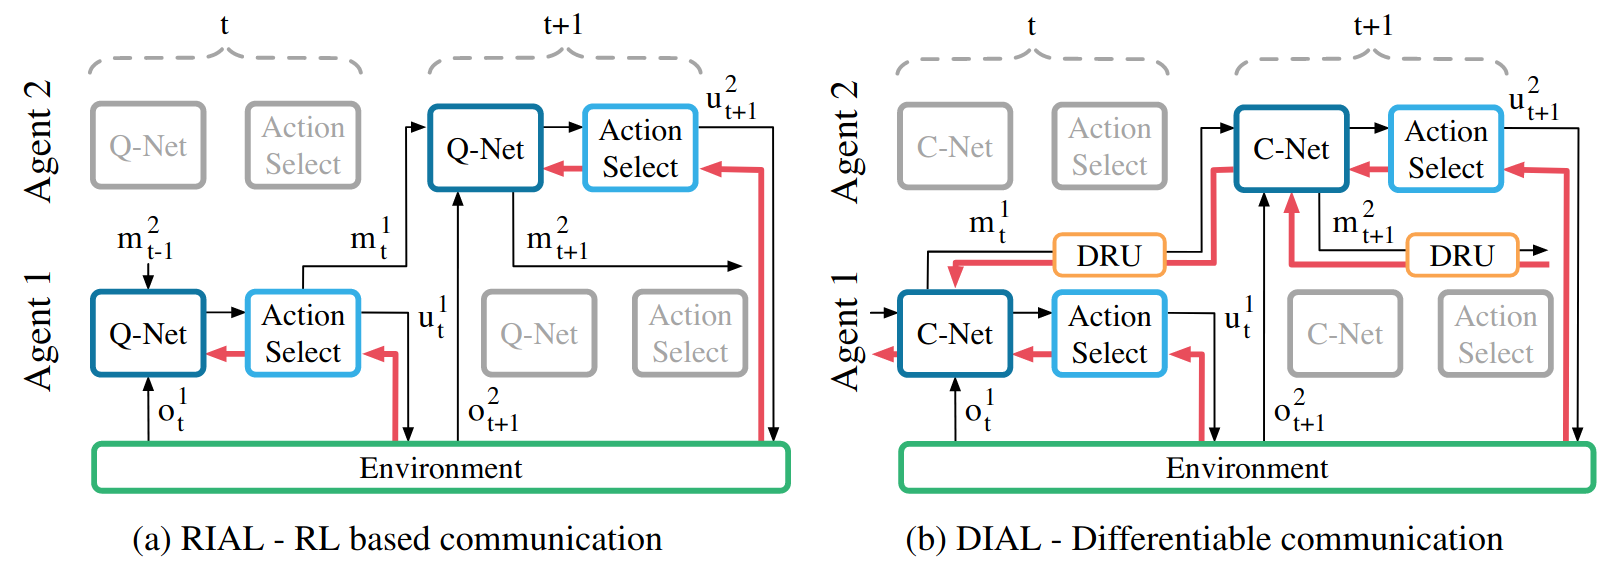
\includegraphics[width=12.1cm]{fig1.png}    
    
    \subsubsection{RIAL}
    \begin{enumerate}
        \item An agent receives observations from the environment and if applicable, any messages from other agents.
        \item This information is inputted into 2 DQNs, which is represented by Q-Net. These two DQNs output values.
        \item The action select (such as $\epsilon$-greedy) will pick which environment action to take and will select which communication action to take based on the outputs of the DQNs (1 DQN each).
        \item Rewards are received and then backpropagation happens, each agent's actions are updated based on their reward from the environment. (there is no information shared on "how good" communication actions were)
    \end{enumerate}
    
    \subsubsection{DIAL}

    \paragraph{Extract} \emph{During centralised learning, communication actions are replaced with direct connections between the output of one agent's network and the input of another agent's. Thus, while the task restricts communication to discrete messages, during learning the agents are free to send real-valued messages to each other}

    \paragraph{Interpretation} The neural network behaves differently during \emph{centralised learning} vs. \emph{decentralised execution} as during the learning process it can send/receive more granular communication instructions (real valued communication vectors). This is allowed by the behaviour of the DRU (explained later).

    \paragraph{C-Net} The C-Net is a really is a network which outputs two values:
    \begin{enumerate}
        \item[$Q(\cdot)$] The Q-values as a normal DQN might. This is fed into the action selector and an \emph{environment action} is chosen.
        \item[$m^a_t$] A real valued vector message to send to other agents. For example: $\begin{bmatrix} 0.44 & 1.45 & 22.42 & -0.2 & 1.0 & -0.01 \end{bmatrix}$. This is sent to the DRU.
    \end{enumerate}
    \paragraph{\emph{Discretise/Regularise Unit} (DRU)} The DRU will operate differently depending on whether it is in the \emph{centralised learning} or \emph{decentralised execution} phase. 
      
    \begin{enumerate}
        \item[centralised learning.] $\text{DRU}(m^a_t) = \text{Logistic}(\mathcal{N}(m^a_t, \sigma))$
        \item[decentralised execution.] $\text{DRU}(m^a_t) = \mathds{1} \{ m^a_t > 0 \}$
    \end{enumerate}
    
    \paragraph{Important note}
    Because during centralised learning the DRU is differentiable, the gradient term for $m$ is the backpropagated error from the recipient of the message to the sender.
    
    \paragraph{Why add the noise?} It "encourages" the model to naturally learn to "discretise" messages during training. This is because if one agent wants to clearly communicate a message $m^a_t$ should either be very high or very low (think: 1 or 0) otherwise after noise is applied the output may be unclear.
    \begin{enumerate}
        \item add noise to the message $m^a_t$ 
        \item apply logistic function to noised message $\mathcal{N}(m^a_t, \sigma)$
        \item send the result $\text{Logistic}(\mathcal{N}(m^a_t, \sigma))$
    \end{enumerate}

    \paragraph{} If you consider that input values of $m^a_t$ which are close to 0 will output a highly uncertain value (because the noise could have a large impact on the output)

    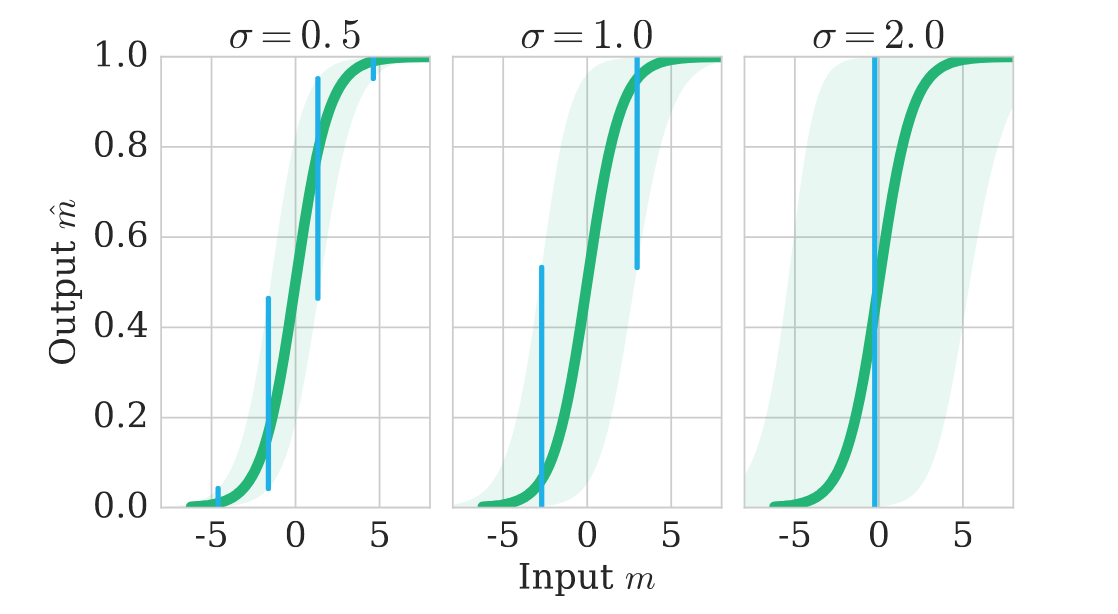
\includegraphics[width=12cm]{fig2.png}
    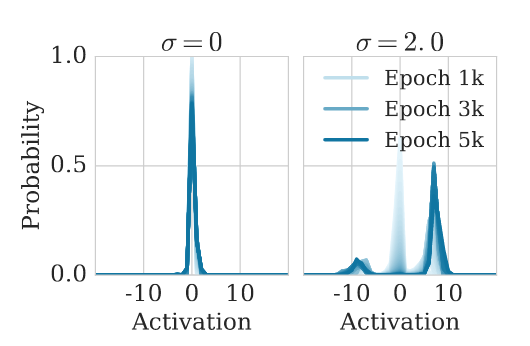
\includegraphics[width=12cm]{fig3.png}
    \section{Their Experiments and Comments}

    \subsection{Switch Riddle}
    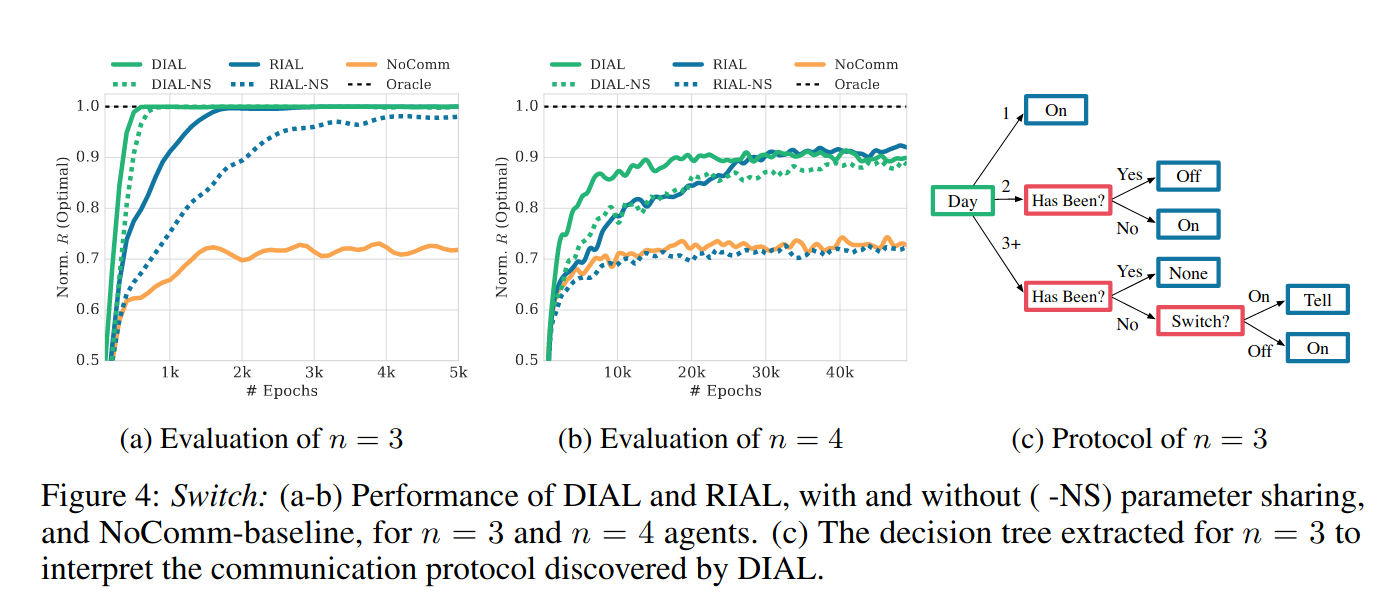
\includegraphics[width=12cm]{fig4.png}

    \paragraph{} DIAL converges much faster than RIAL, however it seems like they tend to have similar performance when there is a low number of agents in the environment. It would be nice to see how they compare when the number of agents is increased.
    \paragraph{Their Github:} https://github.com/iassael/learning-to-communicate

\end{document}